
\chapter[Justificativa da Abordagem]{Justificativa da Abordagem}

\tab A partir da dećada de 1970, a mudança tecnológica  possibilitou um crescimento exorbitante dos recursos de hardware e permitiram que produtos com tecnologias mais avançadas fossem criadas. Entretanto, as tećnicas utilizadas no desenvolvimento  de software não acompanharam o crescimento dos recursos de hardware, este fenômeno ficou conhecido com a Crise de Software. Neste âmbito, Dijkstra destaca:\\

\begin{quote}
	\textsl
	{
		A maior causa da crise do software é que as máquinas tornaram-
		se várias ordens de magnitude mais potentes! Em termos diretos,
		enquanto não havia máquinas, programar não era um problema;
		quando tivemos computadores fracos, isso se tornou um problema
		pequeno e agora que temos computadores gigantescos, programar
		tornou-se um problema gigantesco.
	}
\end{quote}


\tab Não obstante,  ao longo dos anos, notou-se o aumento de metodologias de produção de software com objetivo de aumentar a qualidade e eficiência neste processo. A IEEE define metodologias de desenvolvimento de software como uma abordagem sistemática obtida na etapa de desenvolvimento, no qual, o papel do engenheiro é assegurar que sejam realizadas as melhores escolhas naquele determinado contexto. Vale ressaltar, que estas escolhas têm implicações diretas no sucesso ou fracasso de um projeto.\\

\tab Na etapa de seleção de metodologia foi utilizada o fluxograma proposto pela empresa de consultoria Fortezza Consulting [N]. Apresentado abaixo: \\ 


\begin{figure}[h]
	\centering
	\label{fig01}
		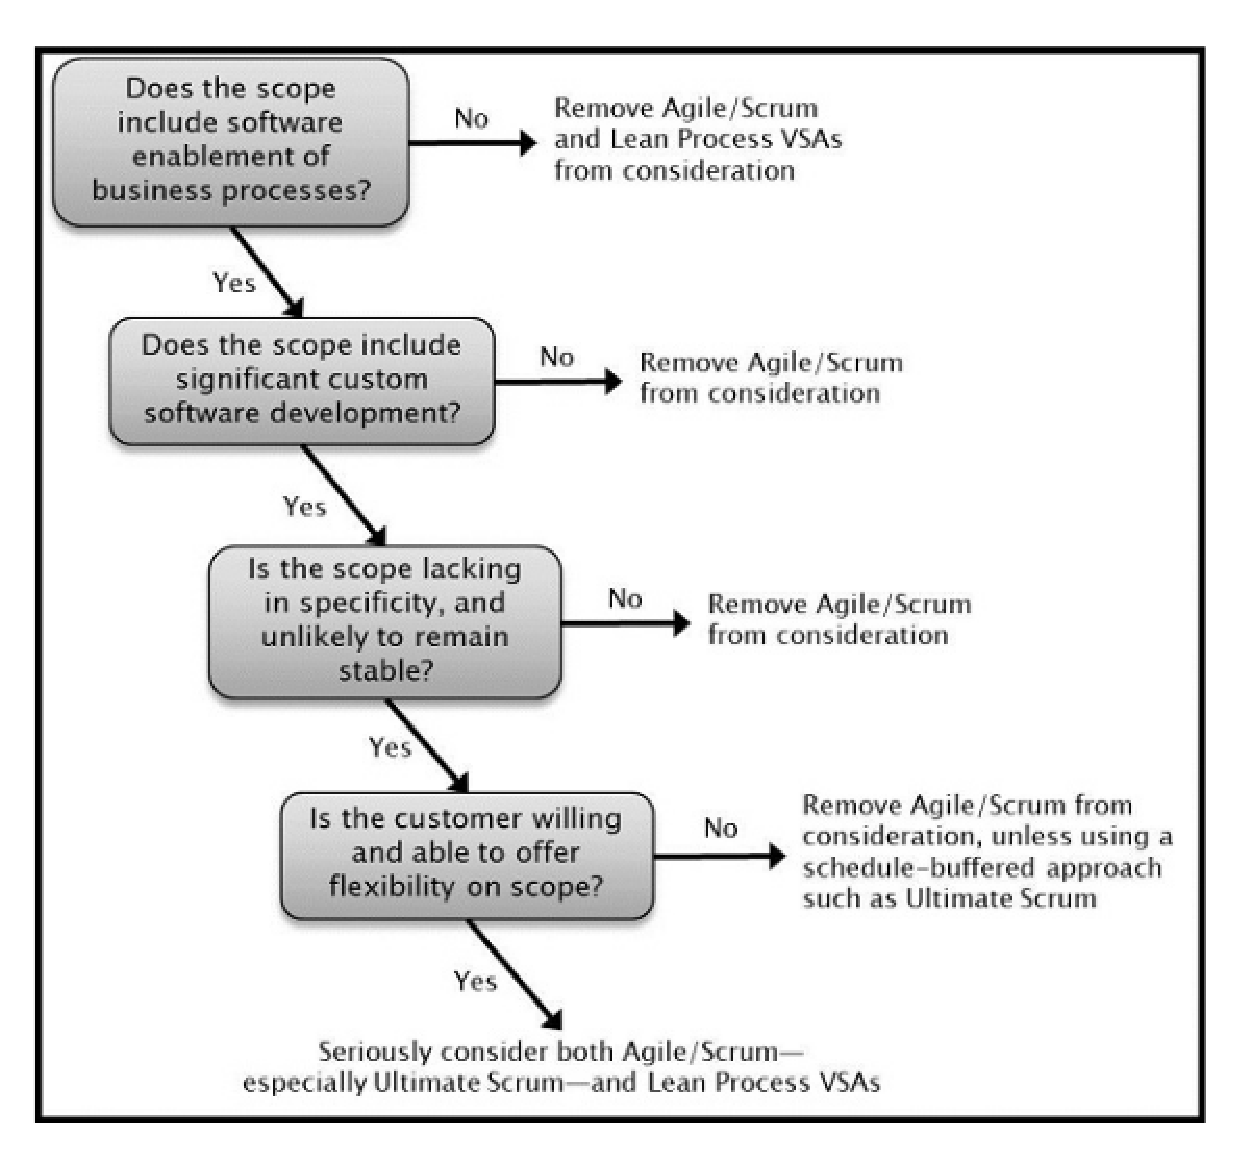
\includegraphics[keepaspectratio=true,scale=0.6]{figuras/fluxograma1.eps}
	\caption{Fluxograma para determinar metodologia a ser utilizada}
\end{figure}


\tab Desta forma, foram considerada as seguintes perguntas: \\

\begin{enumerate}
	\item \textsl{“Does the scope include software enablement of business processes?”} 
	\item \textsl{“Does the scope include software enablement of business processes?”}
	\item \textsl{“Is the scope lacking in specificity, and unlikely to remain stable?”} 
	\item \textsl{“Is the customer willing and able to offer flexibility on scope?”} 
\end{enumerate}

\tab Com base nas respostas das perguntas acima, foi identificada que a metodologia ágil se adaptaria melhor ao nosso contexto.  

\tab Além disso, uma série de fatores que justificaram o emprego da metodologia ágil, os quais estão descritos abaixo:

\begin{enumerate}
	\item {Flexibilidade a mudanças;} 
	\item {Comunicação com o cliente;}
	\item {Planejamento;} 
	\item {Equipe de desenvolvedores;}
	\item {Tamanho do Projeto;}
\end{enumerate}


\large{Flexibilidade a mudanças\\}


O cliente, dono da fábrica de massas “Chef Nery”, ainda não alcançou uma idéia final concreta sobre o sistema que deseja adquirir. Os requisitos, embora já bem direcionados, permanecem instáveis no que diz respeito à definição de utilidades – ainda não é muito certo tudo o que será essencial ou apenas “bom ter” no projeto. Diante tal contexto, é natural que também o cliente esteja predisposto a flexibilizar o escopo da aplicação, permitindo que se assentem gradualmente as diretrizes definitivas do sistema. \\
\tab Esta característica é favorável ao uso de metodologias ágeis, que preveem mudanças constantes no escopo e espera flexibilidade dos cliente envolvido (BECK, 2001). \\

\large{Comunicação com o cliente\\}

\tab O manifesto ágil, criado por  em 1997, propõe uma série de princípios. Dentre eles, destaca-se a interação entre indivíduos como sendo mais relevante que os processos e ferramentas  (BECK, 2001). Assim,  é necessário que os indivíduos tenham uma comunicação bastante próxima  com o cliente e que as interações com o mesmo possam propiciar mudanças e evolução constantes, possibilitando  a obtenção de requisitos voláteis. \\
\tab O pequeno tamanho da equipe, que é formada por apenas 4 estudantes de Engenharia de Software e o cliente, somado ao fato de o cliente estar apto e disposto a participar de reuniões e atender as necessidades da equipe de desenvolvimento, possibilita a comunicação próxima da qual as metodologias ágeis se beneficiam. Para tanto, foram adotadas algumas ferramentas de comunicação como o WhatsApp e Hangouts (para situações de impossibilidade de encontros físicos ou necessidade de reuniões emergenciais). \\


\large{Planejamento\\}

\tab Em metodologias ágeis, usualmente, as equipes economizam um tempo significativo com o planejamento, visto que as interações que ocorrem junto ao cliente fornecem feedbacks constantes. A título de comparação, em metodologias tradicionais aproximadamente 20 por cento do tempo é gasto na etapas de planejamento e replanejamento (BOEHM, 2009). \\
\tab Não obstante, o cliente em nosso contexto não exige documentação expressiva, pelo contrário valoriza as interações provenientes da metodologia ágil. Desta forma, neste contexto  específico é mais interessante adoção da metodologia ágil,  pois esta  possibilita uma economia de recursos e tempo. \\


\large{Equipe de desenvolvedores\\

\tab A equipe de projetistas e desenvolvedores (que, na verdade, é a mesma equipe) já possui melhor familiaridade com metodologias ágeis, compreendendo relativamente bem suas etapas e rituais. \\
\tab Somado a isto, há o tamanho diminuto da equipe, que consta 4 integrantes e o cliente, o que possibilita e também facilita uma comunicação intensa e frequente dos integrantes entre si e com o cliente. \\
\tab Estas características tendem a uma menor dependência de formalidades em documentações e grande dinamicidade na gerência da equipe – ambos fatores que favorecem o uso de metodologias ágeis (AMBLER, 2001). \\

\large{Tamanho do Projeto\\}

\tab De acordo com o manifesto ágil, é necessário que os indivíduos tenham uma comunicação bastante próxima com o cliente (BECK et al, 2001). Não obstante, em projetos menores a comunicação é privilegiada visto a maior interação entre os integrantes do projeto. \\
\tab Além disso, deve-se destacar que em projetos mais complexos, usualmente,  é preferível a utilização de metodologias híbridas ou tradicionais, visto que estas detalham e documentam de forma mais precisa os processos e subprocessos. \\
\tab Em projetos menores este formalismo é menos relevante, pois existe uma comunicação e um feedback maior entre os envolvidos. \\

\large{Scaled Agile Framework(SAFe)\\}

\tab O SAFe  tem como objetivo sintetizar certos conceitos do corpo do conhecimento e as lições aprendidas de centenas de desenvolvimentos de projetos  dentro de um um único framework, a partir dos seguintes valores:\\

\begin{enumerate}
	\item {Alinhamento (Alignment);} 
	\item {Transparência (Transparency);}
	\item {Execução do Programa (Program execution);} 
	\item {Qualidade(Built-in quality);}
\end{enumerate}

\tab Assim, este framework escalável tem como objetivo prover práticas providas de metodologias aǵeis, tais como SCRUM e XP em projetos. Além disso, este framework provém artefatos, documentos e atividades e pode ser dividido em três níveis: Portfólio, Programa e Time.\\
\tab A partir destas características, foi escolhido o SAFe 4.0 ao nosso contexto. Entretanto, foram realizadas algumas adaptações para serem adaptadas ao nosso contexto. Vale ressaltar que o SAFe 4.0 propõe o Value Stream, o qual não foi considerado na elaboração do nosso processo, visto  o tamanho e a simplicidade do projeto \\

\begin{figure}[h]
	\centering
	\label{fig01}
		\includegraphics[keepaspectratio=true,scale=0.5]{figuras/ProcessoSAFE69.eps}
	\caption{Processo}
\end{figure}
